\documentclass[tikz,border=2pt]{standalone}
\usepackage{amsmath,amssymb}
\usepackage{tikz}
\usetikzlibrary{arrows.meta,matrix}

\begin{document}
% A permutation matrix has a single 1 in every row and column; multiplying a vector by it
% just reorders the entries.
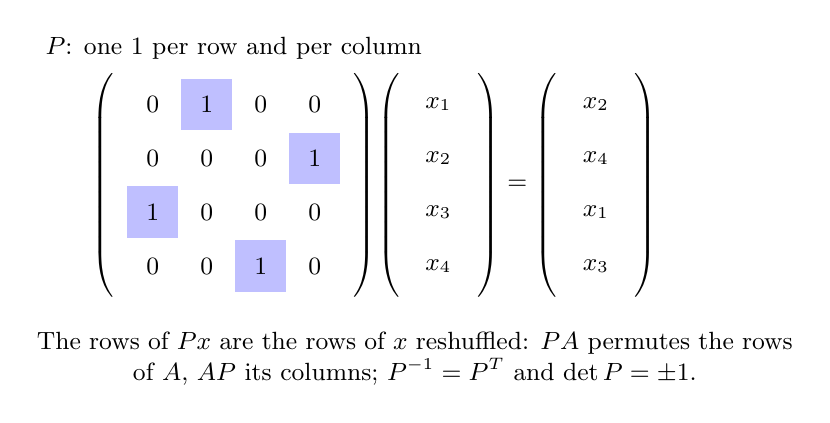
\begin{tikzpicture}[every node/.style={font=\small}]
	\matrix (P) [matrix of math nodes, nodes={minimum size=6.5mm, anchor=center}, left delimiter=(, right delimiter=), column sep=1pt, row sep=1pt] at (0,0) {
		0 & |[fill=blue!25]| 1 & 0 & 0 \\
		0 & 0 & 0 & |[fill=blue!25]| 1 \\
		|[fill=blue!25]| 1 & 0 & 0 & 0 \\
		0 & 0 & |[fill=blue!25]| 1 & 0 \\
	};
	\matrix (x) [matrix of math nodes, nodes={minimum size=6.5mm, anchor=center}, left delimiter=(, right delimiter=), column sep=1pt, row sep=1pt] at (2.6,0) {
		x_1 \\ x_2 \\ x_3 \\ x_4 \\
	};
	\node at (3.6,0) {$=$};
	\matrix (y) [matrix of math nodes, nodes={minimum size=6.5mm, anchor=center}, left delimiter=(, right delimiter=), column sep=1pt, row sep=1pt] at (4.6,0) {
		x_2 \\ x_4 \\ x_1 \\ x_3 \\
	};
	\node[anchor=south] at (P.north) {$P$: one $1$ per row and per column};
	\node[anchor=north, align=flush center, text width=9.6cm] at (2.3,-1.75) {The rows of $Px$ are the rows of $x$ reshuffled: $PA$ permutes the rows of $A$, $AP$ its columns; $P^{-1}=P^{T}$ and $\det P=\pm1$.};
\end{tikzpicture}
\end{document}
